\documentclass[]{article}
\usepackage{lmodern}
\usepackage{amssymb,amsmath}
\usepackage{ifxetex,ifluatex}
\usepackage{fixltx2e} % provides \textsubscript
\ifnum 0\ifxetex 1\fi\ifluatex 1\fi=0 % if pdftex
  \usepackage[T1]{fontenc}
  \usepackage[utf8]{inputenc}
\else % if luatex or xelatex
  \ifxetex
    \usepackage{mathspec}
  \else
    \usepackage{fontspec}
  \fi
  \defaultfontfeatures{Ligatures=TeX,Scale=MatchLowercase}
\fi
% use upquote if available, for straight quotes in verbatim environments
\IfFileExists{upquote.sty}{\usepackage{upquote}}{}
% use microtype if available
\IfFileExists{microtype.sty}{%
\usepackage{microtype}
\UseMicrotypeSet[protrusion]{basicmath} % disable protrusion for tt fonts
}{}
\usepackage[margin=1in]{geometry}
\usepackage{hyperref}
\hypersetup{unicode=true,
            pdftitle={case1final},
            pdfauthor={Nathaniel Brown, Annie Tang, William Yang},
            pdfborder={0 0 0},
            breaklinks=true}
\urlstyle{same}  % don't use monospace font for urls
\usepackage{longtable,booktabs}
\usepackage{graphicx,grffile}
\makeatletter
\def\maxwidth{\ifdim\Gin@nat@width>\linewidth\linewidth\else\Gin@nat@width\fi}
\def\maxheight{\ifdim\Gin@nat@height>\textheight\textheight\else\Gin@nat@height\fi}
\makeatother
% Scale images if necessary, so that they will not overflow the page
% margins by default, and it is still possible to overwrite the defaults
% using explicit options in \includegraphics[width, height, ...]{}
\setkeys{Gin}{width=\maxwidth,height=\maxheight,keepaspectratio}
\IfFileExists{parskip.sty}{%
\usepackage{parskip}
}{% else
\setlength{\parindent}{0pt}
\setlength{\parskip}{6pt plus 2pt minus 1pt}
}
\setlength{\emergencystretch}{3em}  % prevent overfull lines
\providecommand{\tightlist}{%
  \setlength{\itemsep}{0pt}\setlength{\parskip}{0pt}}
\setcounter{secnumdepth}{0}
% Redefines (sub)paragraphs to behave more like sections
\ifx\paragraph\undefined\else
\let\oldparagraph\paragraph
\renewcommand{\paragraph}[1]{\oldparagraph{#1}\mbox{}}
\fi
\ifx\subparagraph\undefined\else
\let\oldsubparagraph\subparagraph
\renewcommand{\subparagraph}[1]{\oldsubparagraph{#1}\mbox{}}
\fi

%%% Use protect on footnotes to avoid problems with footnotes in titles
\let\rmarkdownfootnote\footnote%
\def\footnote{\protect\rmarkdownfootnote}

%%% Change title format to be more compact
\usepackage{titling}

% Create subtitle command for use in maketitle
\newcommand{\subtitle}[1]{
  \posttitle{
    \begin{center}\large#1\end{center}
    }
}

\setlength{\droptitle}{-2em}
  \title{case1final}
  \pretitle{\vspace{\droptitle}\centering\huge}
  \posttitle{\par}
  \author{Nathaniel Brown, Annie Tang, William Yang}
  \preauthor{\centering\large\emph}
  \postauthor{\par}
  \predate{\centering\large\emph}
  \postdate{\par}
  \date{September 13, 2017}


\begin{document}
\maketitle

\subsubsection{Introduction}\label{introduction}

\section{UNFINISHED!!!}\label{unfinished}

The purpose of this project is to analyze rat bioassays. is there
variation in results between labs? there shouldn't be.

\subsubsection{Model-Fitting}\label{model-fitting}

\section{UNFINISHED!!!}\label{unfinished-1}

We fit models to try to understand the variation between labs. Our
approaches were univariate normal, multivariate normal, and mixed
effects.

\paragraph{First Approach: Univariate
Normal}\label{first-approach-univariate-normal}

\[
log(y) \sim \text{Norm}(\mu , \sigma^2)
\]

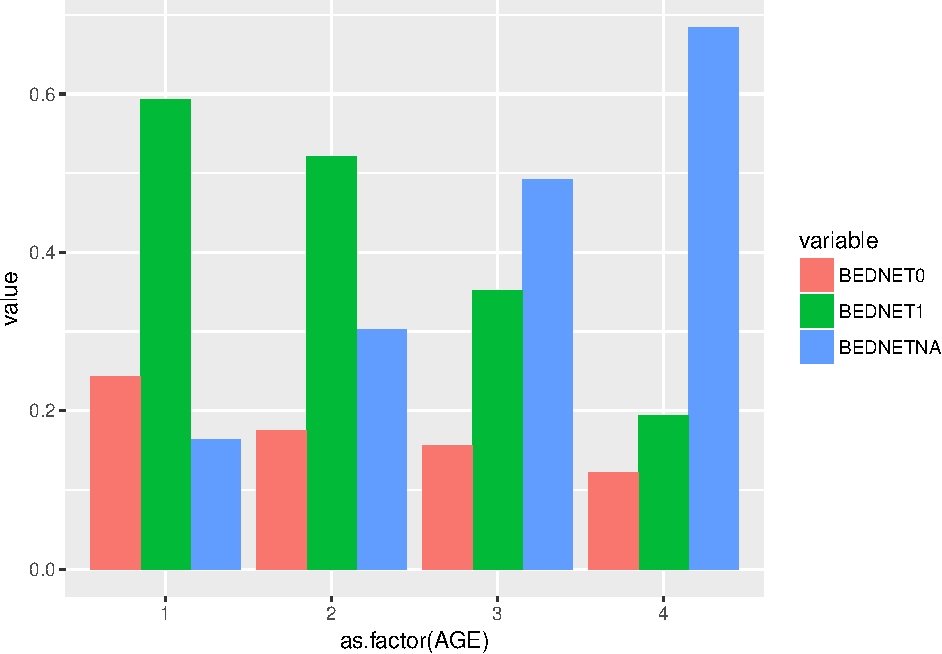
\includegraphics{case1final_files/figure-latex/unnamed-chunk-2-1.pdf}

This naive approach assumes the blotted weight follows a normal
distribution with a mean centered around the mean of the log blotted
weight (4.2619) and constant variance. The diagnostic plots below show
that the same value is predicted for each input, the quantiles of the
residuals do not follow a normal distrbution, and that the residuals are
bimodal. We believe bimodality may be caused by the separation of rats
into juvenille and adult protocols.

\paragraph{Second Approach: Multivariate
Normal}\label{second-approach-multivariate-normal}

\[
y_i, \mu \in M_{n_i \times 1}( \Re)
\\
\Sigma \in M_{n \times n}( \Re)
\\ 
log(y_i) \sim \text{MVNorm}(\mu, \Sigma)
\]

In this model,\(y_i\) is a vector of \(n_i\) observations from lab
\(i\). It assumes that the log blotted weights of each lab follow
approximately normal distributions with a their own means.

We provide the diagnosis plots for the first lab, \texttt{Basf}, and we
put the others in Appendix 1.1, since R does not support plotting for
multivariate regression models.

\begin{verbatim}
## Warning: package 'bindrcpp' was built under R version 3.3.3
\end{verbatim}

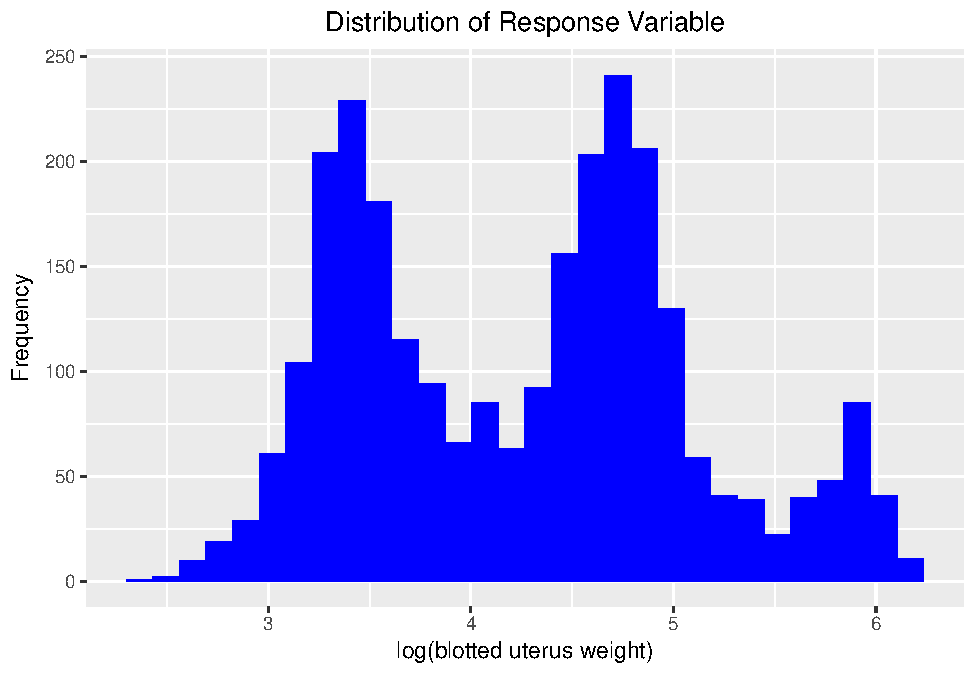
\includegraphics{case1final_files/figure-latex/unnamed-chunk-4-1.pdf}

The diagnostic plots for this model indicate that the model predicts the
same fitted value for each lab, and that the residual quantiles do not
follow a normal distribution. For the \texttt{Basf} lab, the histogram
of residuals shows left skew. These same problems, along with
multimodality of the residuals, are present for the diagnostic plots for
the remaining labs in the Appendix.

A weakness of this model is that, as you add more structure (blocking
factors, covariates for dosage, etc.) to the model, the covariance
matrix becomes more complicated, and maximum likelihood estimation
becomes unwieldy. The poor fit of this model indicates that we should
control for more than just the lab effect, so we consider a mixed
effects model.

\paragraph{Third Approach: Mixed
Effects}\label{third-approach-mixed-effects}

\[
y_{ij} \sim \beta_{0,i} + \beta_{1,i}x_{ij,d_1} + \beta_{2,i}x_{ij,d_2} + \beta_{3,i}x_{ij,p_B} + \beta_{4,i}x_{ij,p_C} + \beta_{5,i}x_{ij,p_D} + \beta_{6,i}x_{ij,log(w)} + \epsilon
\\
\beta_{0:6,i} \sim N(\mu_{0:6,i}, \sigma^2_{0:6,i})
\\
\epsilon \sim N(0, \sigma^2)
\]

Let \(y_{ij}\) be the observation for log(blotted uterus weight) for
subject \(x_{ij}\), the \(j\)th individual in lab \(i\). \(x_{ij,d_1}\)
and \(x_{ij,d_2}\) are the values of dose1 and dose2 for subject
\(x_{ij}\). \(x_{ij,p_B}\), \(x_{ij,p_C}\), and \(x_{ij,p_D}\) are dummy
variables for which protocol \(x_{ij}\) was subjected to.
\(x_{ij,log(w)}\) is the log(body weight) for \(x_{ij}\). We make the
Gaussian assumption that the coefficients, \(\beta\), are normally
distributed according to some \(\mu_i\) and \(\sigma_i\). We add a
random effect on all \(\beta_{0:5,i}\) to account for lab-to-lab
variability in the intercepts and slopes on the blotted weight for the
different dosages and protocols.

We start at a reduced form of this model and augment it to its full form
after initial analyses.

In our analysis, we choose to add a random effect for the lab variable,
in order to account for lab-to-lab heterogeneity. Essentially, this
allows us to avoid violating an independence assumption by assuming a
different baseline response for each lab. First, we model these
differences between individual labs by assuming random intercepts for
each lab. We first include only dose1 and dose2 as fixed effects, then
introduce proto as a fixed effect after confirming through anova (\(p\)
\textless{} 2.2e-16, \(\chi^2\)=1675.8776) that it is a significant
predictor. The summary statistics of this model are shows in the table
below:

\begin{longtable}[]{@{}lrr@{}}
\toprule
& Mean Fixed Effects & Variance Fixed Effects\tabularnewline
\midrule
\endhead
(Intercept) & 3.6311 & 0.0018\tabularnewline
dose1 & 0.1420 & 0.0000\tabularnewline
dose2 & -0.5195 & 0.0012\tabularnewline
protoB & 0.0379 & 0.0008\tabularnewline
protoC & 1.2579 & 0.0009\tabularnewline
protoD & 1.2574 & 0.0016\tabularnewline
\bottomrule
\end{longtable}

\begin{longtable}[]{@{}lrr@{}}
\toprule
& Mean Random Effects & Variance Random Effects\tabularnewline
\midrule
\endhead
(Intercept) & 0.3834 & 0.0284\tabularnewline
\bottomrule
\end{longtable}

\begin{longtable}[]{@{}lr@{}}
\toprule
& Variance\tabularnewline
\midrule
\endhead
Residual & 0.1933\tabularnewline
\bottomrule
\end{longtable}

With this full model, we see that the variability due to lab is 0.028
(in terms of variance), and variability due to non-lab sources is 0.193.
And when we take a look at the fixed effects, we see that an increase in
the amount of dose1 corresponds to an increase (0.142 units) in the
response variable, log(blot). Furthermore, an increase in the amount of
dose2 corresponds to a decrease (-0.519 units) in the response variable.
Protocols B, C, and D all lead to an increase in the response variable,
relative to protocol A. The diagnostic plots below show that this model
fits better than the previous two. Although the residual variance
decreases as the fitted values increase, the quantiles of the residuals
are approximately normal.

\includegraphics{case1final_files/figure-latex/unnamed-chunk-8-1.pdf}

In this random intercept model, we account for baseline differences
between labs, but we also assume that the effects of doses is the same
for each lab. After plotting the log(blot) versus dose by lab, we see
that this is not a valid assumption to make since the lines are clearly
not parallel. So we introduce a random slope model. Now, dose1 and dose2
can have varying slopes.

\includegraphics{case1final_files/figure-latex/unnamed-chunk-9-1.pdf}
\includegraphics{case1final_files/figure-latex/unnamed-chunk-9-2.pdf}

After adding the random slopes, we transformed dose 1 using a reciprocal
transformation and added body weight as a predictor in order to have the
best fitting model. We evaluate this model using summary statistics,
diagnostic plots, and out-of-sample predictive accuracy, which we
evaluate using Mean Absolute Error \((\text{MAE} = E[|y - \hat{y}|])\)
and Root Mean Squared Error
\((\text{RMSE} = \sqrt{E[(y - \hat{y})^2]})\). Root Mean Squared Error
penalizes more for extreme errors, while Mean Absolute Error simply
averages all of the errors.

\begin{longtable}[]{@{}lrr@{}}
\toprule
& Mean Fixed Effects & Variance Fixed Effects\tabularnewline
\midrule
\endhead
(Intercept) & 2.6379 & 0.0728\tabularnewline
protoB & 0.0457 & 0.0003\tabularnewline
protoC & 0.8553 & 0.0094\tabularnewline
protoD & 0.8524 & 0.0100\tabularnewline
log(body) & 0.2946 & 0.0046\tabularnewline
\bottomrule
\end{longtable}

\begin{longtable}[]{@{}lrr@{}}
\toprule
& Mean Random Effects & Variance Random Effects\tabularnewline
\midrule
\endhead
(Intercept) & 3.4691 & 0.9593\tabularnewline
I(1/(dose1 + 1/2)) & 0.4969 & 0.5371\tabularnewline
dose2 & 0.7532 & 1.0481\tabularnewline
\bottomrule
\end{longtable}

\begin{longtable}[]{@{}lr@{}}
\toprule
& Variance\tabularnewline
\midrule
\endhead
Residual & 0.0797\tabularnewline
\bottomrule
\end{longtable}

\includegraphics{case1final_files/figure-latex/unnamed-chunk-10-1.pdf}

\begin{longtable}[]{@{}lrr@{}}
\toprule
& MAE & RMSE\tabularnewline
\midrule
\endhead
Random Dose + Transformations & 21.7968 & 37.7587\tabularnewline
Fixed Dose & 35.2341 & 57.9896\tabularnewline
\bottomrule
\end{longtable}

We see that the variability due to sources other than the random effects
is 0.0797 (decreased from 0.193). Also, the diagnostic plots improved,
although it is notable that the residual variance decreases for larger
fitted values. The fixed dose model is also much worse at predicting
than the random dose model with transformations.

\subsubsection{Lab Variation}\label{lab-variation}

\section{INCOMPLETE}\label{incomplete}

The plot below randomly samples dose1 effects and a lab effects (or
intercepts), and plots the results. Since there is so much variance in
the dose1 effects by lab, we say that the bioassay does depend on lab
and thus this study fails miserably.

\subsubsection{Conclusion}\label{conclusion}

Because the dose 1 effect has such a high variance relative to the mean,
our model shows that the bioassay being studied does not measure a
consistent response to dosage across labs.

\subsubsection{Contributions}\label{contributions}

Nathaniel Brown made the visualizations for this report. He also
organized the relevant files in a Github repository for the group to
access and edit. Annie Tang compiled the group work done on EDA into a
.rmd and wrote the accompanying explanations for the EDA and approaches
to analysis. William Yang helped pair on EDA analysis and identify
approaches to handle the data. Approaches to analysis were a joint
effort by all members of the group. Nathanial implemented analysis for
the univariate normal and multivariate normal approaches. Implementation
and analysis of the mixed effects model was a joint effort by all
members of the group.

\subsubsection{Appendix}\label{appendix}

\paragraph{1.1: Multivariate Normal Diagnosis
Plots}\label{multivariate-normal-diagnosis-plots}

\includegraphics{case1final_files/figure-latex/unnamed-chunk-12-1.pdf}
\includegraphics{case1final_files/figure-latex/unnamed-chunk-12-2.pdf}
\includegraphics{case1final_files/figure-latex/unnamed-chunk-12-3.pdf}
\includegraphics{case1final_files/figure-latex/unnamed-chunk-12-4.pdf}
\includegraphics{case1final_files/figure-latex/unnamed-chunk-12-5.pdf}
\includegraphics{case1final_files/figure-latex/unnamed-chunk-12-6.pdf}
\includegraphics{case1final_files/figure-latex/unnamed-chunk-12-7.pdf}
\includegraphics{case1final_files/figure-latex/unnamed-chunk-12-8.pdf}
\includegraphics{case1final_files/figure-latex/unnamed-chunk-12-9.pdf}
\includegraphics{case1final_files/figure-latex/unnamed-chunk-12-10.pdf}
\includegraphics{case1final_files/figure-latex/unnamed-chunk-12-11.pdf}
\includegraphics{case1final_files/figure-latex/unnamed-chunk-12-12.pdf}
\includegraphics{case1final_files/figure-latex/unnamed-chunk-12-13.pdf}
\includegraphics{case1final_files/figure-latex/unnamed-chunk-12-14.pdf}
\includegraphics{case1final_files/figure-latex/unnamed-chunk-12-15.pdf}
\includegraphics{case1final_files/figure-latex/unnamed-chunk-12-16.pdf}
\includegraphics{case1final_files/figure-latex/unnamed-chunk-12-17.pdf}
\includegraphics{case1final_files/figure-latex/unnamed-chunk-12-18.pdf}


\end{document}
